% fancytikzposter.tex, version 2.1
% Original template created by Elena Botoeva [botoeva@inf.unibz.it], June 2012
% 
% This file is distributed under the Creative Commons Attribution-NonCommercial 2.0
% Generic (CC BY-NC 2.0) license
% http://creativecommons.org/licenses/by-nc/2.0/ 


\documentclass{a0poster}

\usepackage{fancytikzposter} 


%%%%% --------- Change here if you want ---------- %%%%%
%% margin for the geometry package, must be changed before using the geometry package
%% default value is 4cm
% \setmargin{4}

%% the space between the blocks
%% default value is 2cm
% \setblockspacing{2}

%% the height of the title stripe in block nodes, decrease it to save space
%% default value is 3cm
% \setblocktitleheight{3}

%% the number of columns in the poster, possible values 2,3
%% default value is 2
% \setcolumnnumber{3}

%% the space between two or more groups of authors from different institutions
%% used in \maketitle
% \setinstituteshift{10}

%% which template to use
%% N1 simple, standard look, with a colored background and gray boxes
%% N2 board with nodes
%% N3 another standard look
%% N4 envelope-like look
%% N5 with a wave-like head, original idea taken from
%%%% http://fc09.deviantart.net/fs71/f/2010/322/1/1/scientific_poster_by_nabuy-d333ria.jpg
%\usetemplate{6}

%% components of the templates
%% (the maximal possible numbers are mentioned as the parameters)
% \usecolortemplate{4}
% \usebackgroundtemplate{5}
% \usetitletemplate{2}
% \useblocknodetemplate{5}
% \useplainblocktemplate{4}
% \useinnerblocktemplate{2}


%% the height of the head drawing on top 
%% applicable to templates N3, 4 and 5
% \setheaddrawingheight{14}


%% change the basic colors
%\definecolor{myblue}{HTML}{008888} 
%\setfirstcolor{myblue}% default 116699
%\setsecondcolor{gray!80!}% default CCCCCC
%\setthirdcolor{red!80!black}% default 991111

%% change the more specific colors
% \setbackgrounddarkcolor{colorone!70!black}
% \setbackgroundlightcolor{colorone!70!}
% \settitletextcolor{textcolor}
% \settitlefillcolor{white}
% \settitledrawcolor{colortwo}
% \setblocktextcolor{textcolor}
% \setblockfillcolor{white}
% \setblocktitletextcolor{colorone}
% \setblocktitlefillcolor{colortwo} %the color of the border
% \setplainblocktextcolor{textcolor}
% \setplainblockfillcolor{colorthree!40!}
% \setplainblocktitletextcolor{textcolor}
% \setplainblocktitlefillcolor{colorthree!60!}
% \setinnerblocktextcolor{textcolor}
% \setinnerblockfillcolor{white}
% \setinnerblocktitletextcolor{white}
% \setinnerblocktitlefillcolor{colorthree}


%%% size of the document and the margins
%% A0
% \usepackage[margin=\margin cm, paperwidth=118.9cm, paperheight=84.1cm]{geometry} 
\usepackage[margin=\margin cm, paperwidth=30in, paperheight=40in]{geometry}
%% B1
% \usepackage[margin=\margin cm, paperwidth=70cm, paperheight=100cm]{geometry}

%% changing the fonts
\usepackage{cmbright}
%\usepackage[default]{cantarell}
%\usepackage{avant}
%\usepackage[math]{iwona}
\usepackage[math]{kurier}
\usepackage[T1]{fontenc}
\usepackage{graphicx}


%% add your packages here
\usepackage{hyperref}
%\usepackage{algorithm}
%\usepackage{ algorithmic}
\usepackage{algpseudocode}
\usepackage{caption}

\title{PowerlineWhisperer}
\author{*Abhinav Narain, Nick Feamster, Mung Chiang, *Matthieu Bloch\\
  Princeton University, *Georgia Tech\\
  \texttt{ anarain@cs.princeton.edu ,feamster@cs.princeton.edu, } \\
  \texttt{mchiang@princeton.edu, bloch@ece.gatech.edu}
}

\begin{document}
%%%%% ---------- the background picture ---------- %%%%%
%% to change it modify the macro \BackgroundPicture
\ClearShipoutPicture
\AddToShipoutPicture{\BackgroundPicture}

\noindent % to have the picture right in the center
\begin{tikzpicture}
  \initializesizeandshifts
  % \setxshift{15}
  % \setyshift{2}
  %% the title block, #1 - shift, the default value is (0,0), #2 - width, #3 - scale
  %% the alias of the title block is `title', so we can refer to its boundaries later
  \ifthenelse{\equal{\template}{1}}{ 
    \titleblock{47}{1}
  }{
    \titleblock{47}{1.5}
  }

  %% a logo can be added to the title block
  %% #1 - anchor relative to the title block, #2 - shift, #3 - width, #3 - file name
  \ifthenelse{\equal{\template}{1}}{ 
   %  \addlogo[south east]{(2,0)}{6cm}{figures/GeorgiaTechSeal.png}
   %  \addlogo[south west]{(2,0)}{6cm}{figures/princetonLogo.png}
  }{
     %\addlogo[south east]{(2,0)}{6cm}{figures/GeorgiaTechSeal.png}
  }


  %% by default, the position of the new block node is right below the previous
  %% block node, stored in (currenty)
  %% box is the alias of the previous block, so we can refer to its boundaries

  %%%%%%%%%% ------------------------------------------ %%%%%%%%%%
  \blocknode{Problem Statement}%
  {
    \innerblock{Purpose}{Allow deniable communication between two parties}
    \begin{center}
    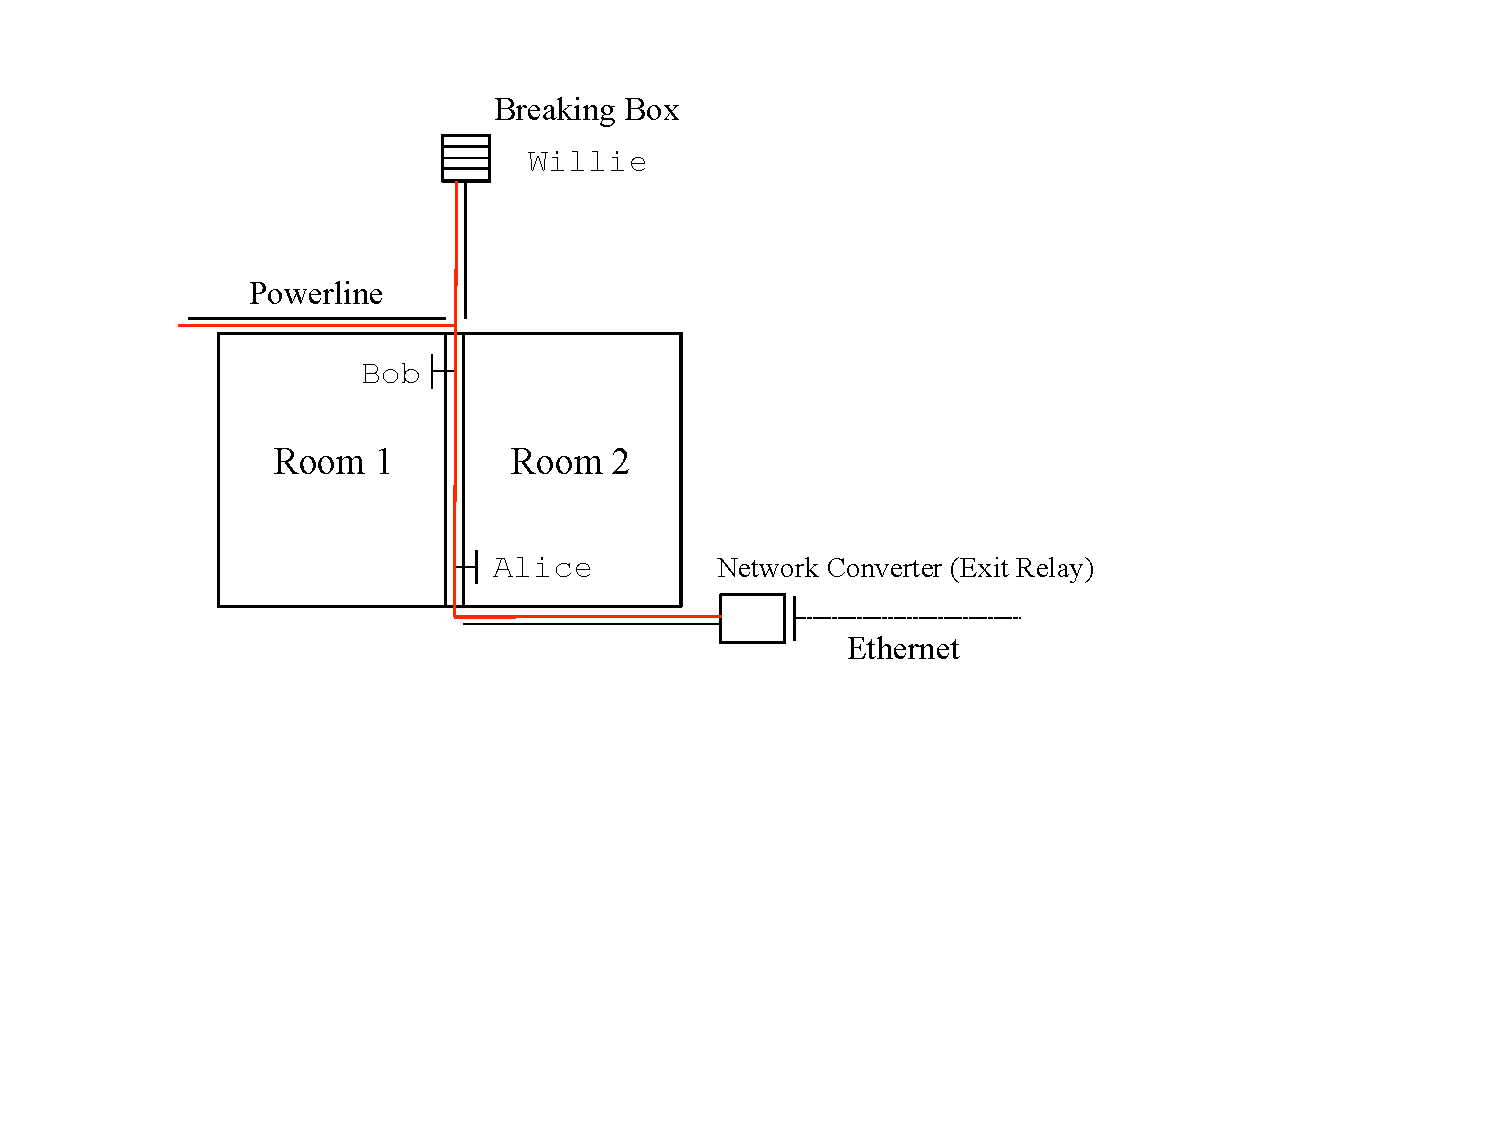
\includegraphics[scale=0.85]{figures/setup.pdf} 
    \end{center}
    
    \innerblock{Approach}{Use ambient noise in public infrastructure}
    \begin{center}
    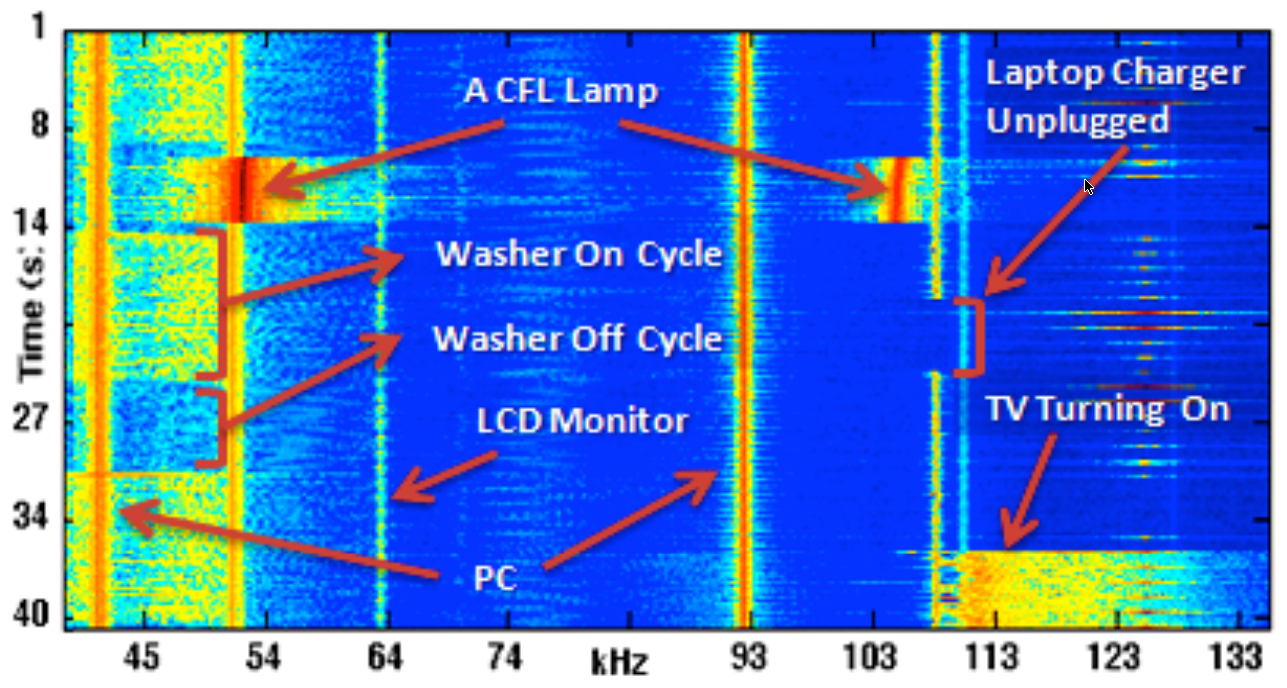
\includegraphics[scale=0.30]{figures/emi.png}
    \end{center}
  }

  \blocknode{Theoretical Framework}%
  {

    \innerblock{Information-theoretic modeling}{
    \begin{center}
    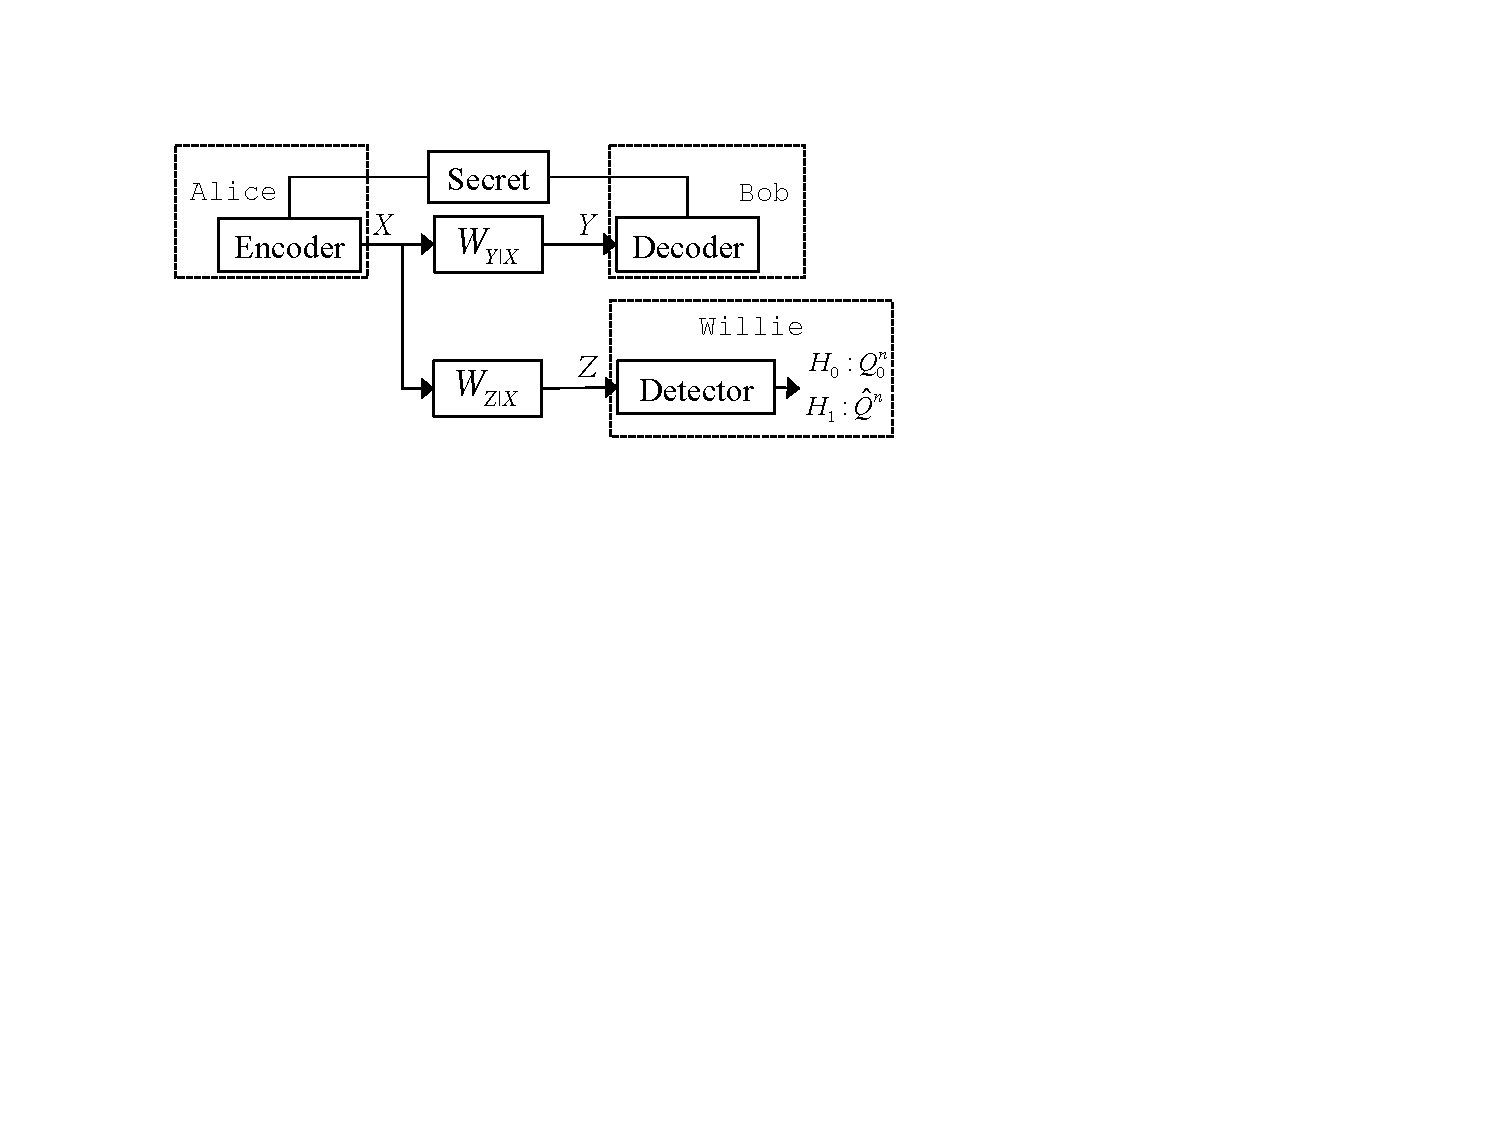
\includegraphics[scale=1.5]{figures/model.pdf} 
    \end{center}
    }


\innerblock{Threat Model} {
    \textbf{Adversary capability}
    \begin{itemize}
      \item Monitoring device to measure quadrature samples at Mains supply of
      physical powerline network 
      \item Unlimited storage capability and ability to do analysis of collected data
    \end{itemize}
    Let the adversary use a hypothesis detector with the following two hypothesis:
    \begin{itemize}
    \item \textbf{$H_{0}$}: Covert communication is \textit{not} happening.
    \item \textbf{$H_{1}$}: Covert communication is  happening.
    \end{itemize}

    Willie's optimal hypothesis test yields the tradeoff \\
    $\alpha + \beta \geq 1 - V(Q_{0}^{n},\hat{Q_{n}})$, \\
    where $V(Q_{0}^{n},\hat{Q_{n}})$ is the variational distance between the true
    distribution (that is of noise) represented by $Q_{0}^{n}$ and estimated
    distribution $\hat{Q_{n}}$, which is in the presence of
    communication.

    \begin{center}
    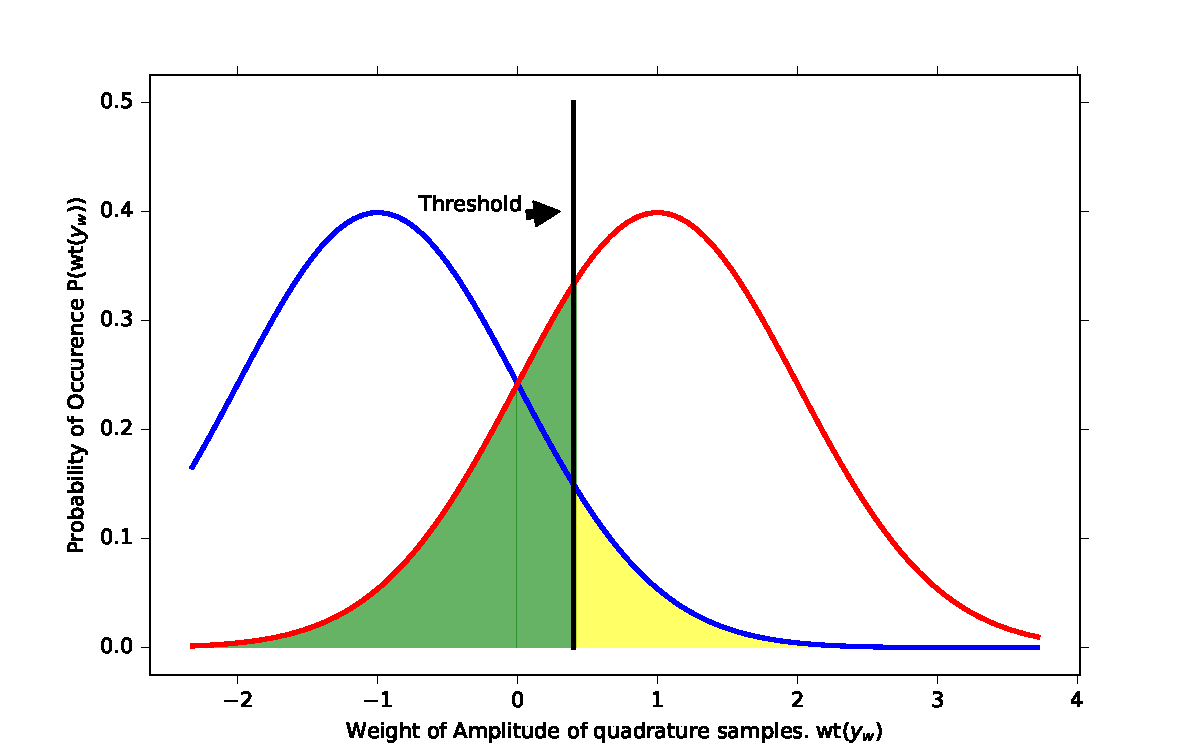
\includegraphics[scale=0.55]{figures/noise.pdf} 
    \end{center}
    }

  }

  %%%%%%%%%%%%% NEW COLUMN %%%%%%%%%%%%%%% 
  \startsecondcolumn 

  %%%%%%%%%% ------------------------------------------ %%%%%%%%%%
  \blocknode{System Design }% 
  {
    \innerblock{Transmission Strategy}{
    %\begin{algorithm}  [H]
    \begin{algorithmic}[1]
      \Procedure{Transmission Slot\textendash Selection}{}\newline
       Initialize the random number generator with the secret key. Let the
       message size be $M$ in number of bits. 
      \For{$1$ \ldots  $M$ } 
         \State {Choose a number from a uniform distribution ($0$,$M^{2}$)
              generated by the random number generator} 
         \State {Place your message bit in the slot}
         \EndFor
         \EndProcedure
            \end{algorithmic}
            Transmit the whole sequence of bits on the channel
     %\end{algorithm}

    }

    \innerblock{Transmitter and Receiver Block Chain} { 
      PowerlineWhisperer implements various blocks in software define
      radio (Gnuradio) for transmitter and receiver

      Transmit chain at the transmitter consists of several blocks which convert
      the original message to waveforms on Powerline \\ 
    \begin{center}
    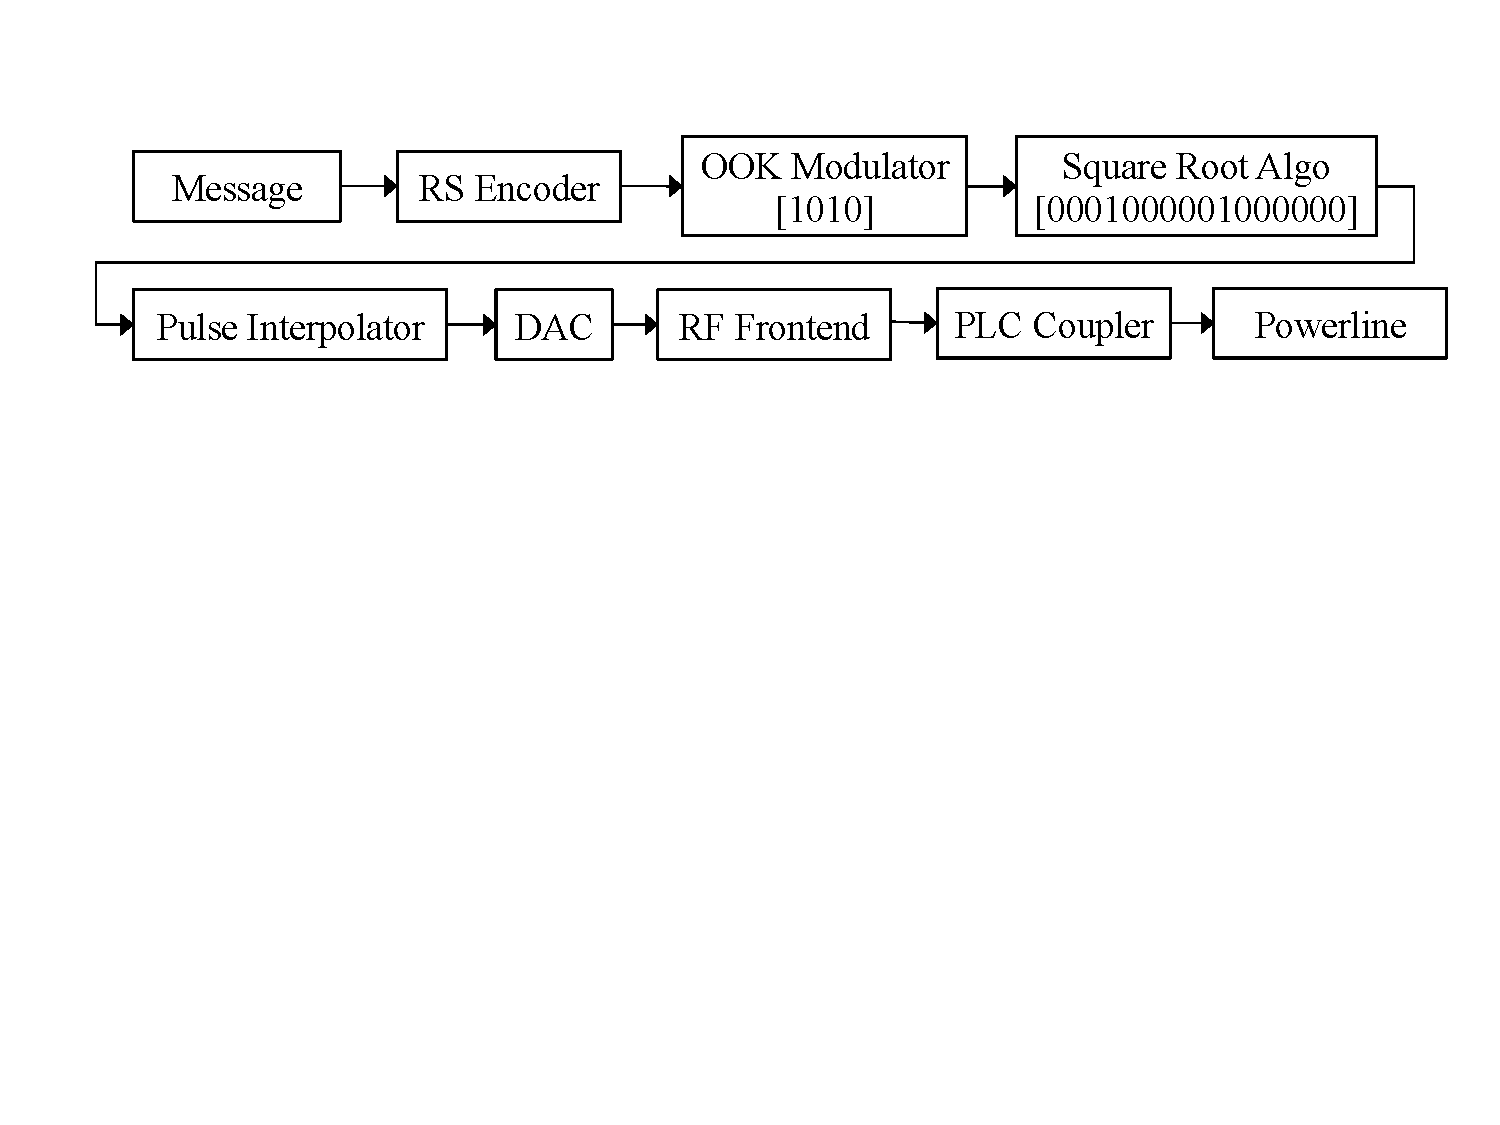
\includegraphics[scale=1.0]{figures/transmitter.pdf} 
      \captionof{figure}{Transmitter Block Chain}
    \end{center}
      Receive chain at the receiver consists of \\
    \begin{center}
    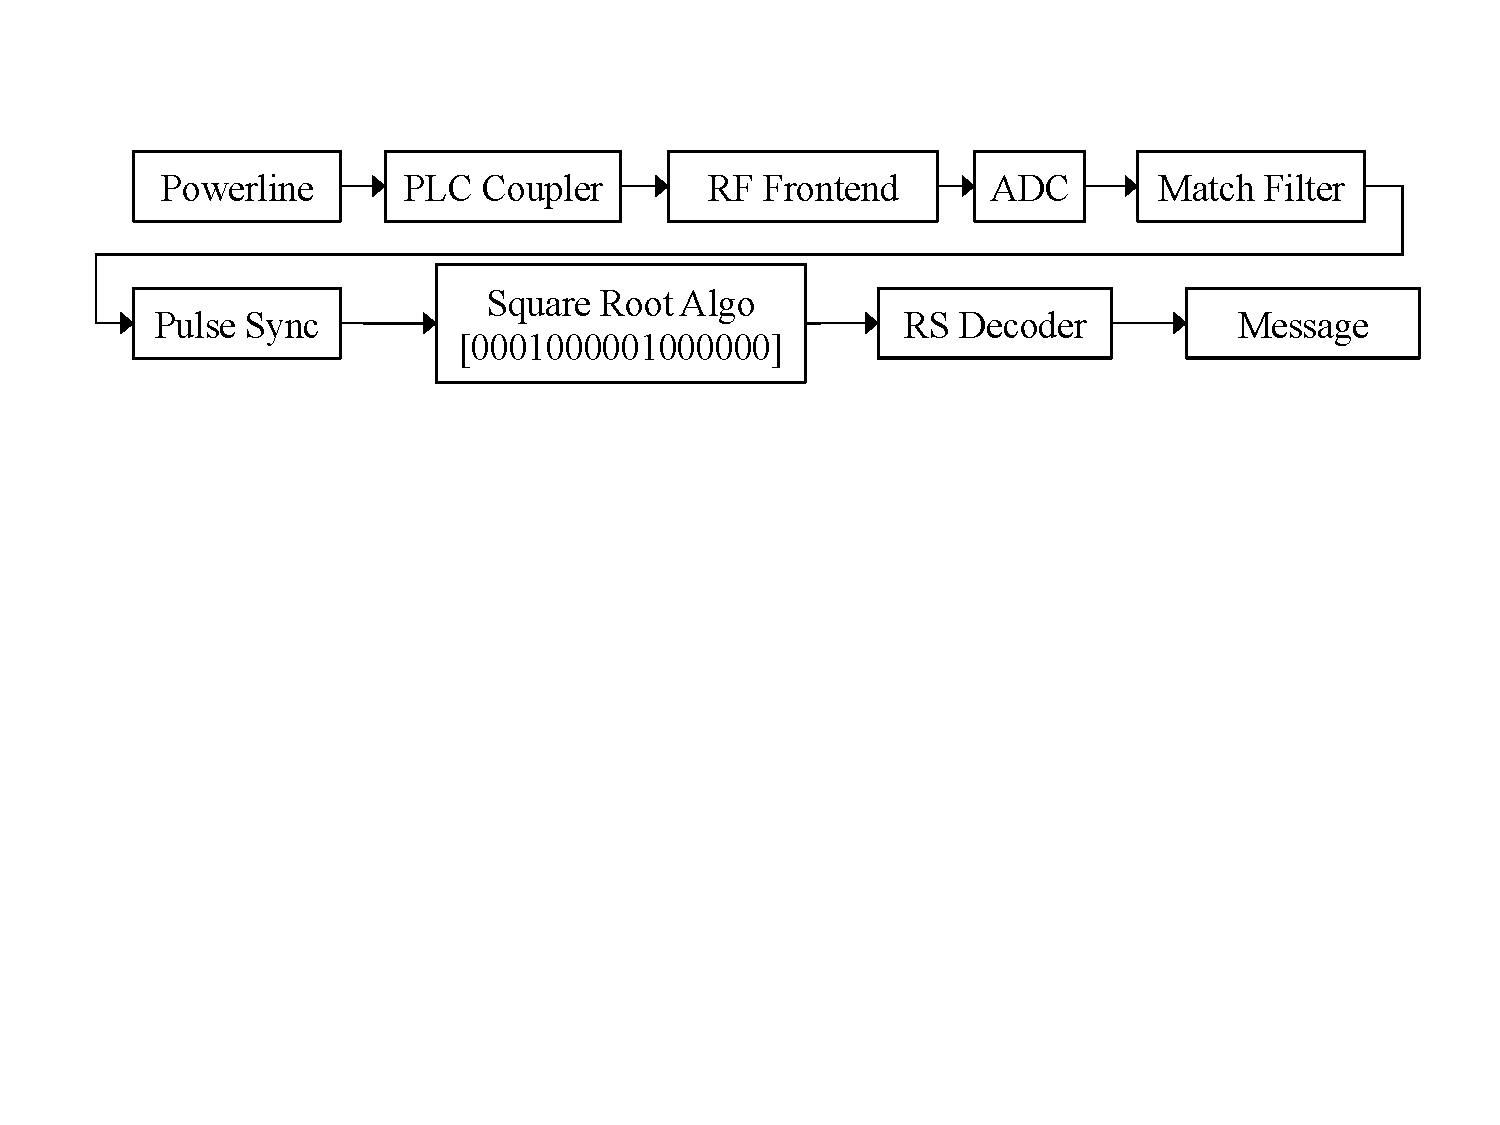
\includegraphics[scale=1.0]{figures/receiver.pdf}
      \captionof{figure}{Receiver Block Chain}
    \end{center}
    }

  }
  %%%%%%%%%% ------------------------------------------ %%%%%%%%%%

  \blocknode{Results}%
  { 
    \innerblock{Adversary Performance}{
    \begin{center}
    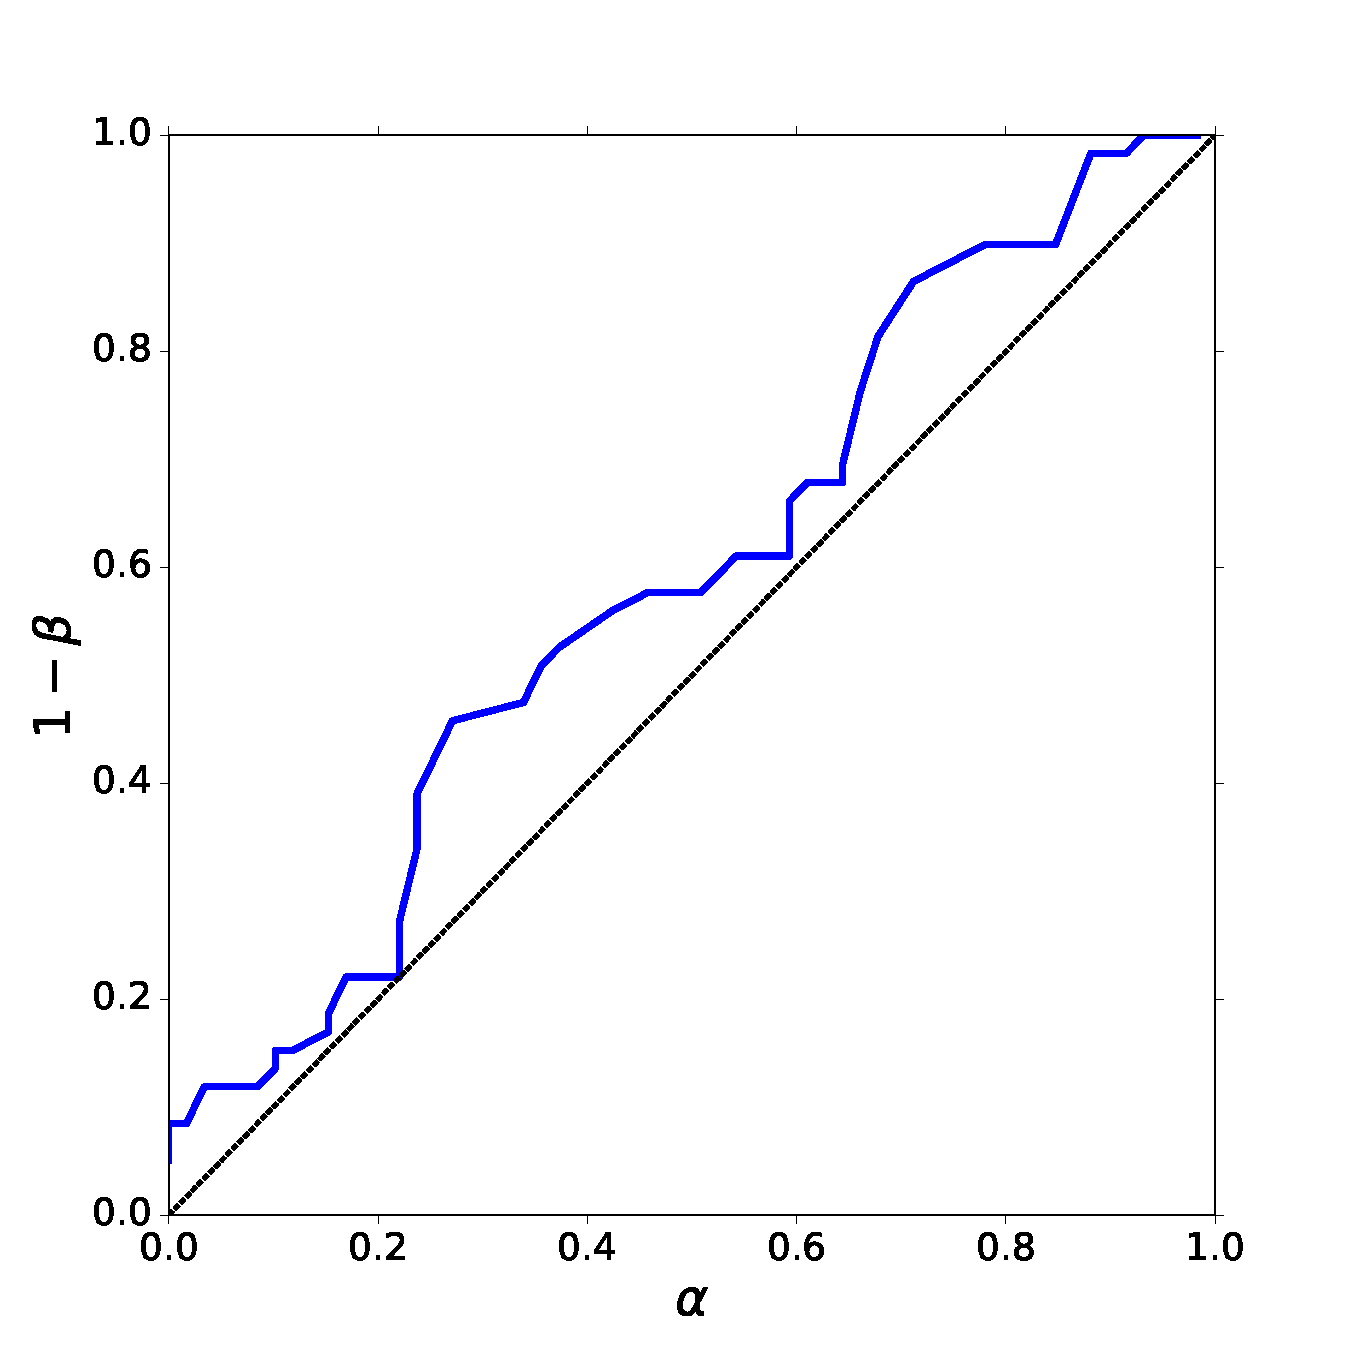
\includegraphics[scale=0.25]{figures/roc_curve.pdf} 
    \end{center}
    \begin{center}
    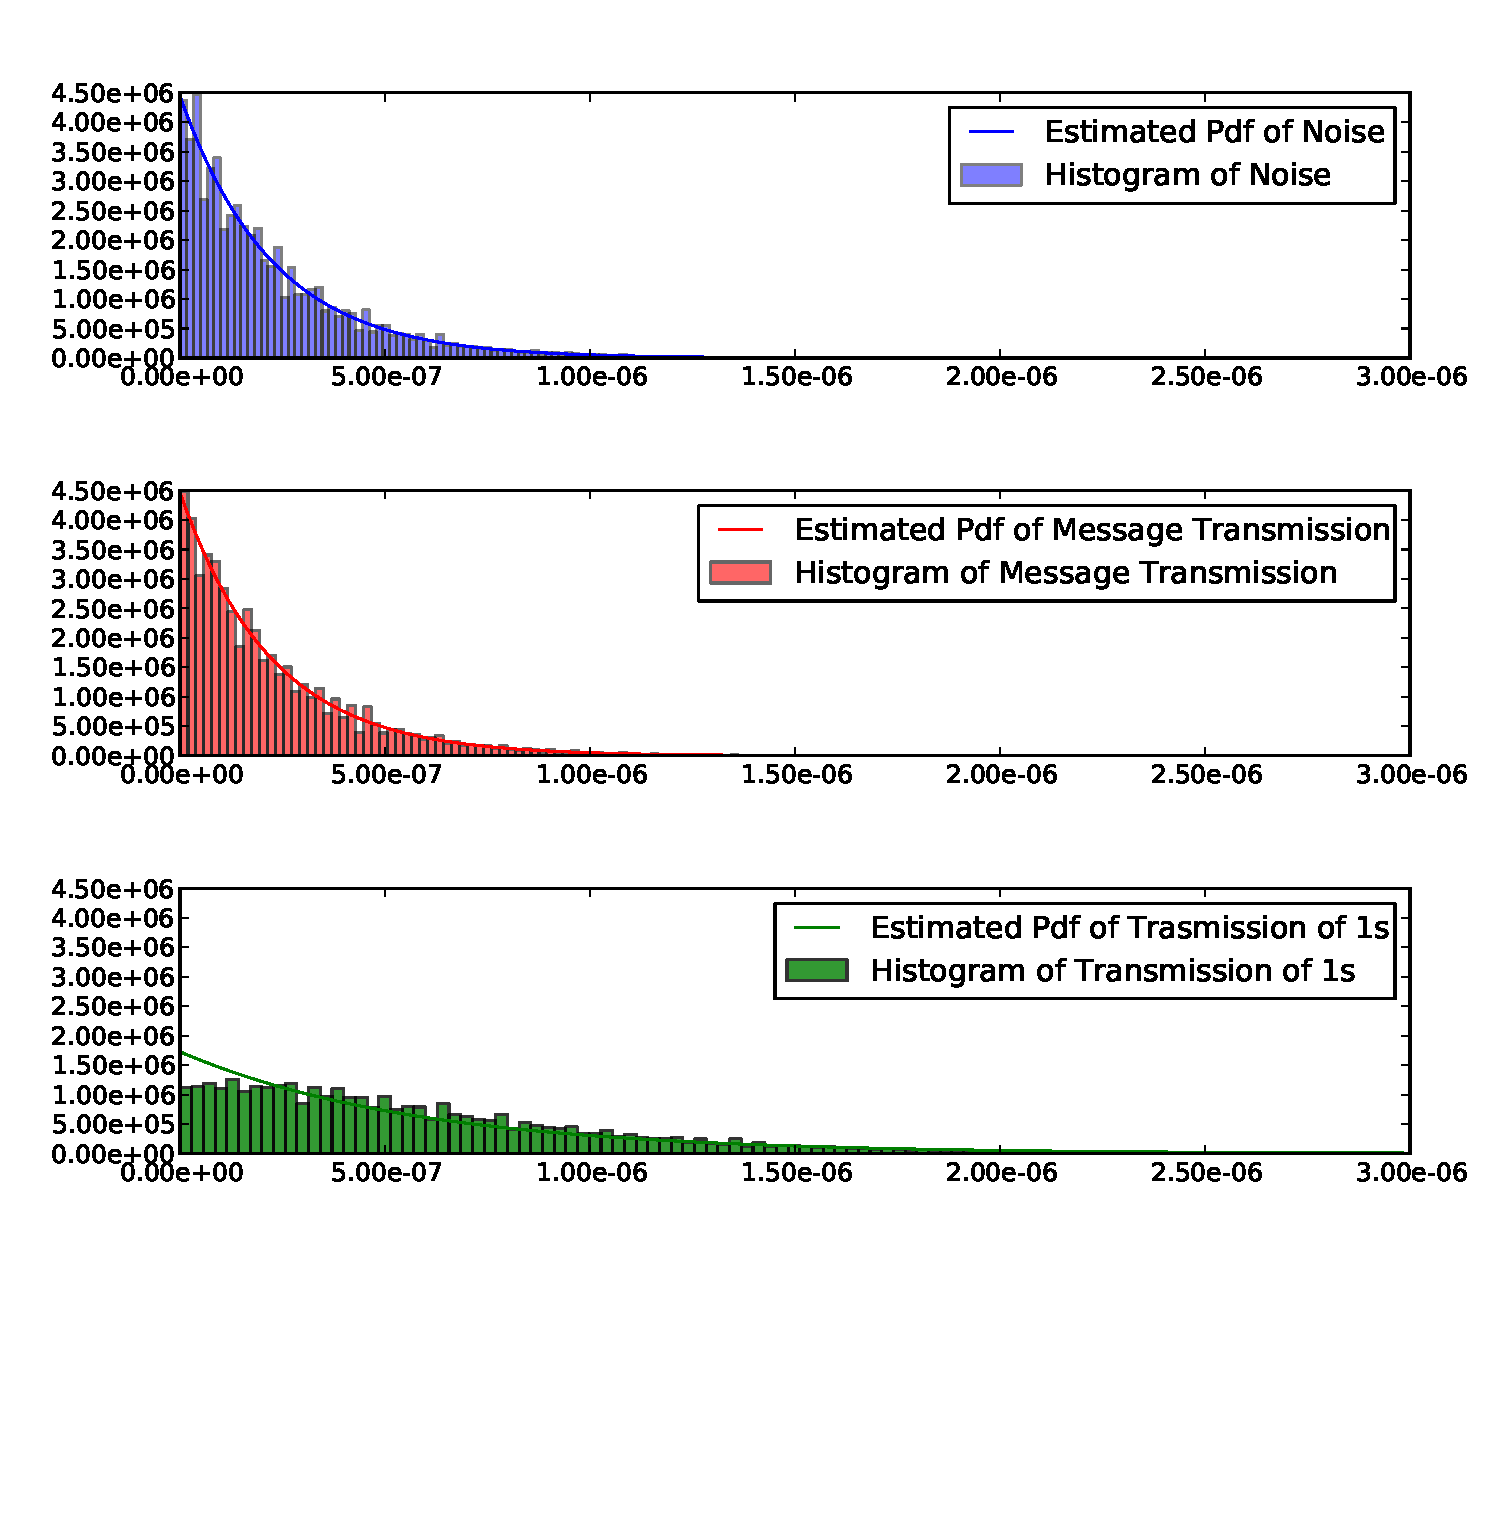
\includegraphics[scale=0.25]{figures/ncurve_53_1_05_iq.pdf}
    \end{center}
    }
  }
  %%%%%%%%%% ------------------------------------------ %%%%%%%%%%

\end{tikzpicture}
\end{document}
